% This file was created with matplot2tikz v0.5.3.
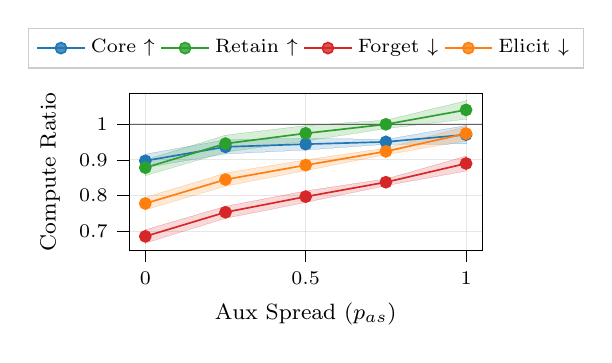
\begin{tikzpicture}

\definecolor{crimson2143940}{RGB}{214,39,40}
\definecolor{darkgray176}{RGB}{176,176,176}
\definecolor{darkorange25512714}{RGB}{255,127,14}
\definecolor{darkslategray77}{RGB}{77,77,77}
\definecolor{forestgreen4416044}{RGB}{44,160,44}
\definecolor{lightgray204}{RGB}{204,204,204}
\definecolor{steelblue31119180}{RGB}{31,119,180}

\begin{axis}[
label style={font=\footnotesize},
tick label style={font=\scriptsize},
title style={font=\footnotesize},
height=3.57cm,
legend cell align={left},
legend columns=4,
legend style={
  font=\scriptsize,
  fill opacity=0.8,
  draw opacity=1,
  text opacity=1,
  at={(0.5,1.16)},
  anchor=south,
  draw=lightgray204
},
tick align=outside,
tick pos=left,
width=0.5\linewidth,
x grid style={darkgray176, opacity=0.3},
xlabel={Aux Spread (\(\displaystyle p_{as}\))},
xmajorgrids,
xmin=-0.05, xmax=1.05,
xtick style={color=black},
y grid style={darkgray176, opacity=0.3},
ylabel={Compute Ratio},
ymajorgrids,
ymin=0.647650499706325, ymax=1.08508456780526,
ytick style={color=black}
]
\path [draw=steelblue31119180, fill=steelblue31119180, opacity=0.18, line width=0pt]
(axis cs:0,0.915882261076119)
--(axis cs:0,0.878573235539218)
--(axis cs:0.25,0.916336878824608)
--(axis cs:0.5,0.927569800010048)
--(axis cs:0.75,0.943386936507252)
--(axis cs:1,0.944419841008663)
--(axis cs:1,0.996092132556909)
--(axis cs:1,0.996092132556909)
--(axis cs:0.75,0.956902200700762)
--(axis cs:0.5,0.95999567784728)
--(axis cs:0.25,0.956066602828828)
--(axis cs:0,0.915882261076119)
--cycle;

\path [draw=forestgreen4416044, fill=forestgreen4416044, opacity=0.18, line width=0pt]
(axis cs:0,0.900074949410945)
--(axis cs:0,0.856083809171292)
--(axis cs:0.25,0.92180792258735)
--(axis cs:0.5,0.952378648619009)
--(axis cs:0.75,0.987560188924968)
--(axis cs:1,1.01369319507826)
--(axis cs:1,1.06520120107349)
--(axis cs:1,1.06520120107349)
--(axis cs:0.75,1.01077992517235)
--(axis cs:0.5,0.995645503882613)
--(axis cs:0.25,0.968775042649953)
--(axis cs:0,0.900074949410945)
--cycle;

\path [draw=crimson2143940, fill=crimson2143940, opacity=0.18, line width=0pt]
(axis cs:0,0.704730282711806)
--(axis cs:0,0.667533866438095)
--(axis cs:0.25,0.73677581676676)
--(axis cs:0.5,0.781128884966609)
--(axis cs:0.75,0.828094772665725)
--(axis cs:1,0.86888679090552)
--(axis cs:1,0.910496876527211)
--(axis cs:1,0.910496876527211)
--(axis cs:0.75,0.846766169868674)
--(axis cs:0.5,0.813025964825197)
--(axis cs:0.25,0.770339198301287)
--(axis cs:0,0.704730282711806)
--cycle;

\path [draw=darkorange25512714, fill=darkorange25512714, opacity=0.18, line width=0pt]
(axis cs:0,0.795328290729602)
--(axis cs:0,0.760641498636672)
--(axis cs:0.25,0.826734151507826)
--(axis cs:0.5,0.870137853708036)
--(axis cs:0.75,0.914479856492001)
--(axis cs:1,0.953056889400817)
--(axis cs:1,0.993559988051619)
--(axis cs:1,0.993559988051619)
--(axis cs:0.75,0.932579400114303)
--(axis cs:0.5,0.90002563994763)
--(axis cs:0.25,0.863110068591205)
--(axis cs:0,0.795328290729602)
--cycle;

\addplot [line width=0.32pt, darkslategray77, opacity=0.85, forget plot]
table {%
-0.05 1
1.05 1
};
\addplot [semithick, steelblue31119180, mark=*, mark size=2, mark options={solid}]
table {%
0 0.897227748307668
0.25 0.936201740826718
0.5 0.943782738928664
0.75 0.950144568604007
1 0.970255986782786
};
\addlegendentry{Core $\uparrow$}
\addplot [semithick, forestgreen4416044, mark=*, mark size=2, mark options={solid}]
table {%
0 0.878079379291118
0.25 0.945291482618651
0.5 0.974012076250811
0.75 0.999170057048658
1 1.03944719807588
};
\addlegendentry{Retain $\uparrow$}
\addplot [semithick, crimson2143940, mark=*, mark size=2, mark options={solid}]
table {%
0 0.68613207457495
0.25 0.753557507534023
0.5 0.797077424895903
0.75 0.837430471267199
1 0.889691833716366
};
\addlegendentry{Forget $\downarrow$}
\addplot [semithick, darkorange25512714, mark=*, mark size=2, mark options={solid}]
table {%
0 0.777984894683137
0.25 0.844922110049516
0.5 0.885081746827833
0.75 0.923529628303152
1 0.973308438726218
};
\addlegendentry{Elicit $\downarrow$}
\end{axis}

\end{tikzpicture}
